%%%%%%%%%%%%%%%%%%%%%%%%%%%%%%%%%%%%%%%%%
% Jacobs Landscape Poster
% LaTeX Template
% Version 1.0 (29/03/13)
%
% Created by:
% Computational Physics and Biophysics Group, Jacobs University
% https://teamwork.jacobs-university.de:8443/confluence/display/CoPandBiG/LaTeX+Poster
% 
% Further modified by:
% Nathaniel Johnston (nathaniel@njohnston.ca)
%
% This template has been downloaded from:
% http://www.LaTeXTemplates.com
%
% License:
% CC BY-NC-SA 3.0 (http://creativecommons.org/licenses/by-nc-sa/3.0/)
%
%%%%%%%%%%%%%%%%%%%%%%%%%%%%%%%%%%%%%%%%%

%----------------------------------------------------------------------------------------
%	PACKAGES AND OTHER DOCUMENT CONFIGURATIONS
%----------------------------------------------------------------------------------------

\documentclass[final]{beamer}

\usepackage[scale=1.24]{beamerposter} % Use the beamerposter package for laying out the poster

\usetheme{confposter} % Use the confposter theme supplied with this template

\setbeamercolor{block title}{fg=ngreen,bg=white} % Colors of the block titles
\setbeamercolor{block body}{fg=black,bg=white} % Colors of the body of blocks
\setbeamercolor{block alerted title}{fg=white,bg=dblue!70} % Colors of the highlighted block titles
\setbeamercolor{block alerted body}{fg=black,bg=dblue!10} % Colors of the body of highlighted blocks
% Many more colors are available for use in beamerthemeconfposter.sty

%-----------------------------------------------------------
% Define the column widths and overall poster size
% To set effective sepwid, onecolwid and twocolwid values, first choose how many columns you want and how much separation you want between columns
% In this template, the separation width chosen is 0.024 of the paper width and a 4-column layout
% onecolwid should therefore be (1-(# of columns+1)*sepwid)/# of columns e.g. (1-(4+1)*0.024)/4 = 0.22
% Set twocolwid to be (2*onecolwid)+sepwid = 0.464
% Set threecolwid to be (3*onecolwid)+2*sepwid = 0.708

\newlength{\sepwid}
\newlength{\onecolwid}
\newlength{\twocolwid}
\newlength{\threecolwid}
\setlength{\paperwidth}{48in} % A0 width: 46.8in
\setlength{\paperheight}{36in} % A0 height: 33.1in
\setlength{\sepwid}{0.024\paperwidth} % Separation width (white space) between columns
\setlength{\onecolwid}{0.22\paperwidth} % Width of one column
\setlength{\twocolwid}{0.464\paperwidth} % Width of two columns
\setlength{\threecolwid}{0.708\paperwidth} % Width of three columns
\setlength{\topmargin}{-0.5in} % Reduce the top margin size
%-----------------------------------------------------------

\usepackage{graphicx}  % Required for including images
\usepackage{booktabs} % Top and bottom rules for tables

%multi-row
\usepackage{multirow}
\usepackage{tikz}

%----------------------------------------------------------------------------------------
%	TITLE SECTION 
%----------------------------------------------------------------------------------------

\title{CS230 - Learning to Play Minichess Without Human Knowledge} % Poster title

\author{Karthik selvakumar Bhuvaneswaran} % Author(s)

\institute{karthik0@stanford.edu} % Institution(s)

%----------------------------------------------------------------------------------------

\begin{document}

\addtobeamertemplate{headline}{} 
{\begin{tikzpicture}[remember picture, overlay]
     \node [anchor=north west, inner sep=3cm]  at (current page.north west)
     {
\includegraphics[height=10cm]{stanford-university-logo.png}};
  \end{tikzpicture}}

\addtobeamertemplate{block end}{}{\vspace*{2ex}} % White space under blocks
\addtobeamertemplate{block alerted end}{}{\vspace*{2ex}} % White space under highlighted (alert) blocks

\setlength{\belowcaptionskip}{2ex} % White space under figures
\setlength\belowdisplayshortskip{2ex} % White space under equations

\begin{frame}[t] % The whole poster is enclosed in one beamer frame

\begin{columns}[t] % The whole poster consists of three major columns, the second of which is split into two columns twice - the [t] option aligns each column's content to the top

\begin{column}{\sepwid}\end{column} % Empty spacer column

\begin{column}{\onecolwid} % The first column

\setbeamercolor{block alerted title}{fg=black,bg=ngreen} % Change the alert block title colors
\setbeamercolor{block alerted body}{fg=black,bg=white} % Change the alert block body colors
%----------------------------------------------------------------------------------------
%	OBJECTIVES
%----------------------------------------------------------------------------------------

\begin{alertblock}{Abstract}

\begin{itemize}
\item Implementing a self play based algorithm using neural nets has become popular after the huge success of Alpha Zero by Deep Mind.
\item Replicating the results for games with larger search space like chess requires scaling. 
\item We develop a scaled up version of alpha-zero-general for the game of Minichess and evaluate our learning algorithm with various baselines.
\end{itemize}
Keywords: \emph{CNN, Reinforcement Learning, Distributed Computing, Monte Carlo search}

\end{alertblock}


%----------------------------------------------------------------------------------------
%	INTRODUCTION
%----------------------------------------------------------------------------------------

\begin{block}{Introduction}

\begin{itemize}
\item Self play and improve without any human knowledge.
\item MCTS provides provides ground truth to compare and learn.
\item 5X5 chess board with Gardner layout will be used for our training. 
\end{itemize}

\begin{figure}
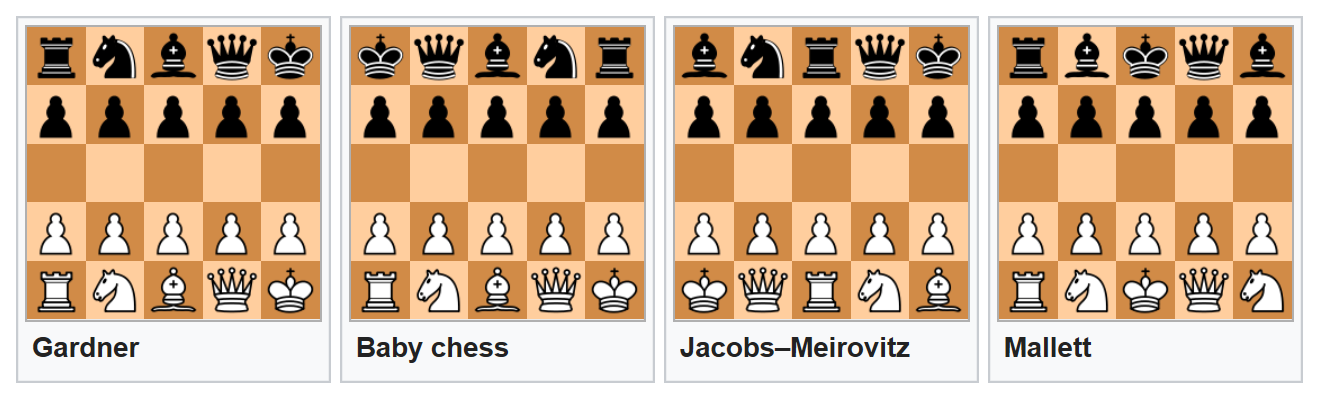
\includegraphics[width=1.0\linewidth]{minichess.png}
\caption{Popular Minichess Board Layouts}
\end{figure}

\begin{itemize}
\item Single Neural network used for both Policy and Value evaluation
\item We will use the following Loss function \[ l = - \sum (v_{\theta}(s_{t}) - z_{t})^{2}+ \vec{\pi_{t}} log(\vec{p_{\theta}}(s_{t}))  \]
\end{itemize}

\begin{figure}
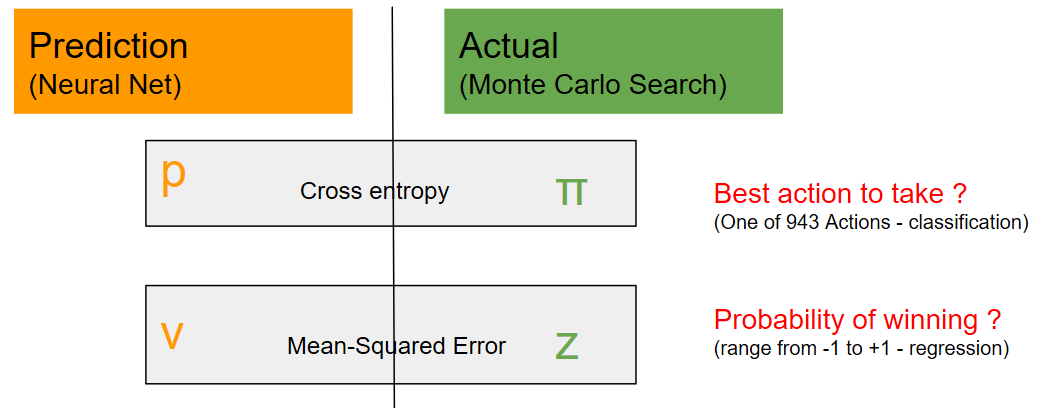
\includegraphics[width=1.0\linewidth]{loss.png}
\caption{Parameters in network and choice of loss functions}
\end{figure}


\end{block}

%------------------------------------------------

%----------------------------------------------------------------------------------------

\end{column} % End of the first column

\begin{column}{\sepwid}\end{column} % Empty spacer column

\begin{column}{\twocolwid} % Begin a column which is two columns wide (column 2)

\begin{columns}[t,totalwidth=\twocolwid] % Split up the two columns wide column

\begin{column}{\onecolwid}\vspace{-.6in} % The first column within column 2 (column 2.1)

%----------------------------------------------------------------------------------------
%	MATERIALS
%----------------------------------------------------------------------------------------

\begin{block}{Distributed Architecture}

Three major components in self play and learn are:

\begin{itemize}
\item \emph{Training Data Generator} - Plays games and generates data for training.
\item \emph{Trainer} - Consumes the data from Training Data Generator, compares against MCTS and learns.
\item \emph{Pitter} - Compares two models and publishes a winner model.
\end{itemize}
\begin{figure}
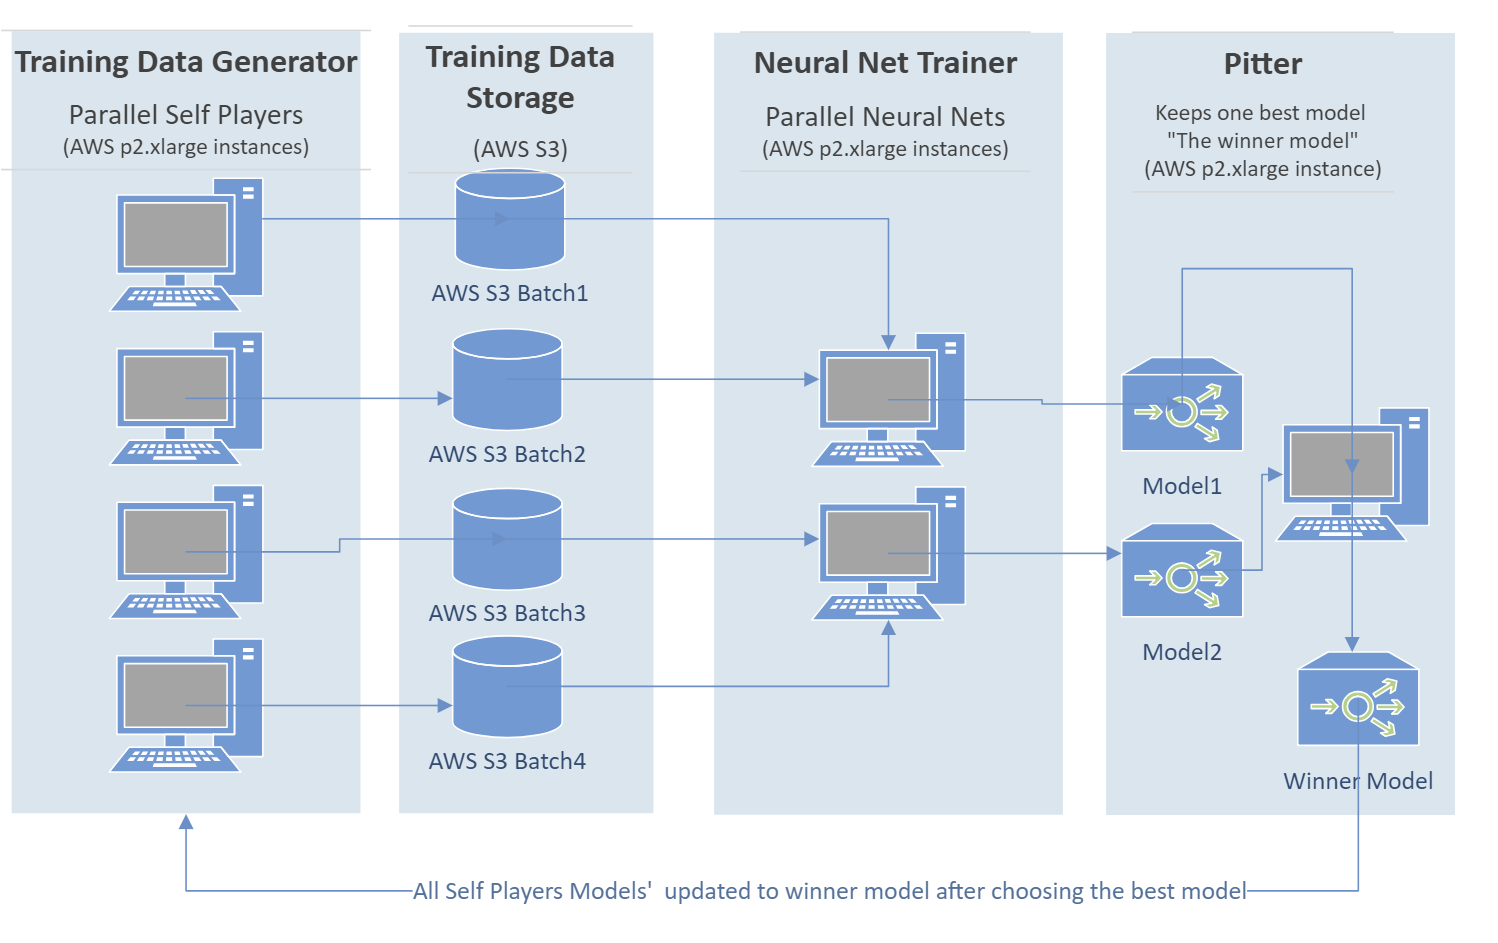
\includegraphics[width=1.0\linewidth]{distributed_arch.png}
\caption{Scaling up the training using Distributed Architecture}
\end{figure}

\end{block}

\begin{column}{\onecolwid} % The first column within column 2 (column 2.1)

%----------------------------------------------------------------------------------------
%	MATHEMATICAL SECTION
%----------------------------------------------------------------------------------------

\begin{block}{Neural Network Model}


\begin{figure}
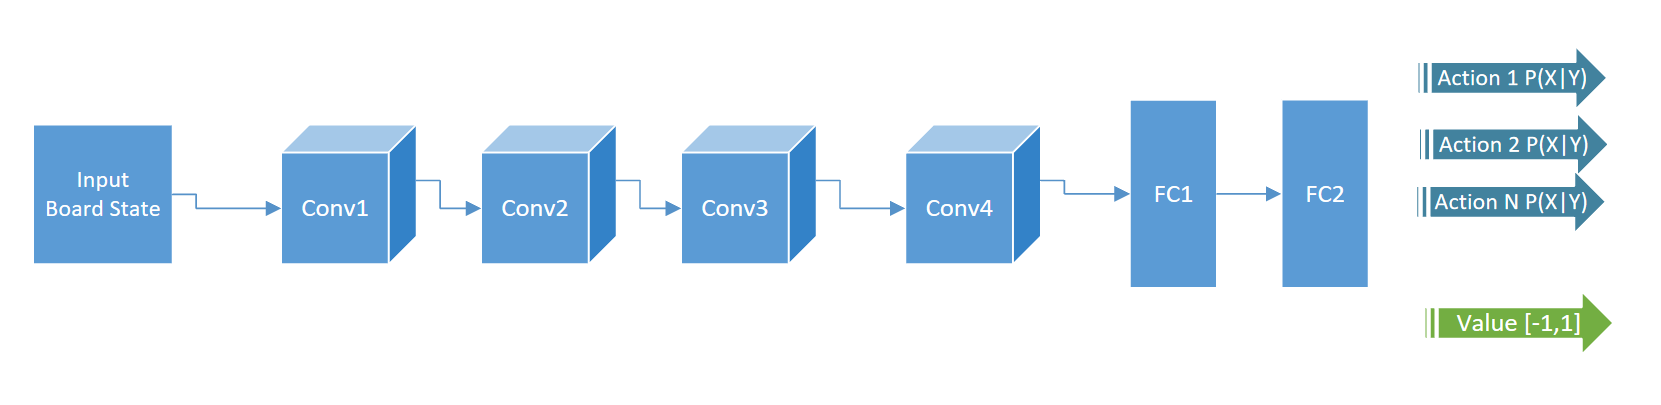
\includegraphics[width=0.8\linewidth]{cnn.png}
\caption{CNN Layers with both Policy and Value output}
\end{figure}

\begin{figure}
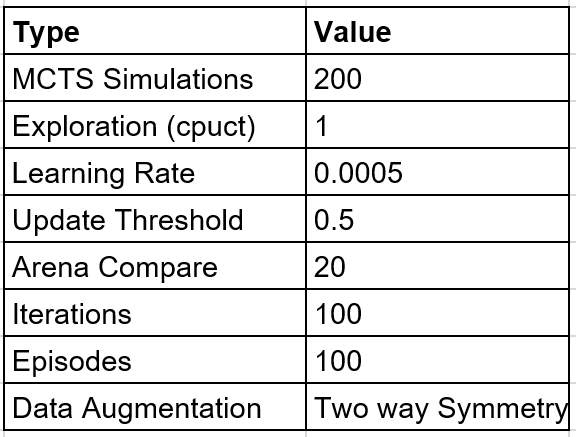
\includegraphics[width=0.4\linewidth]{pre_hyper.png}
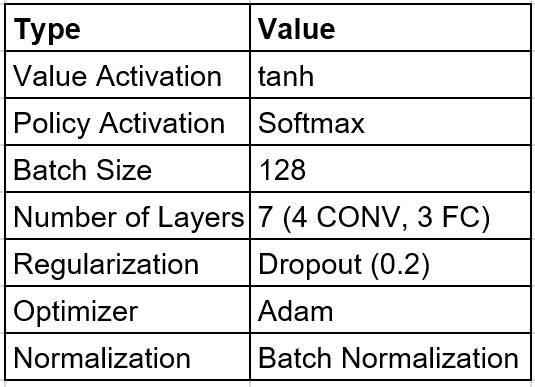
\includegraphics[width=0.4\linewidth]{hyper.png}
\caption{Hyperparams used for Pre-processing and Training}
\end{figure}

\begin{figure}
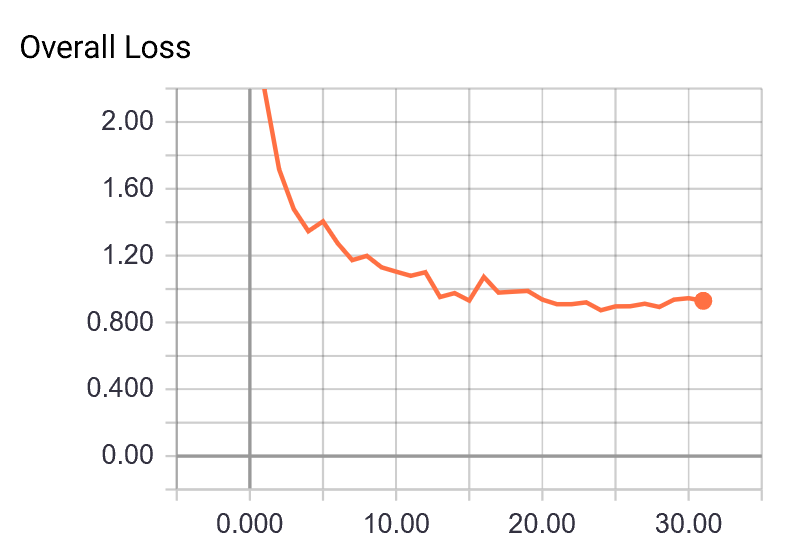
\includegraphics[width=0.3\linewidth]{overall_loss.png}
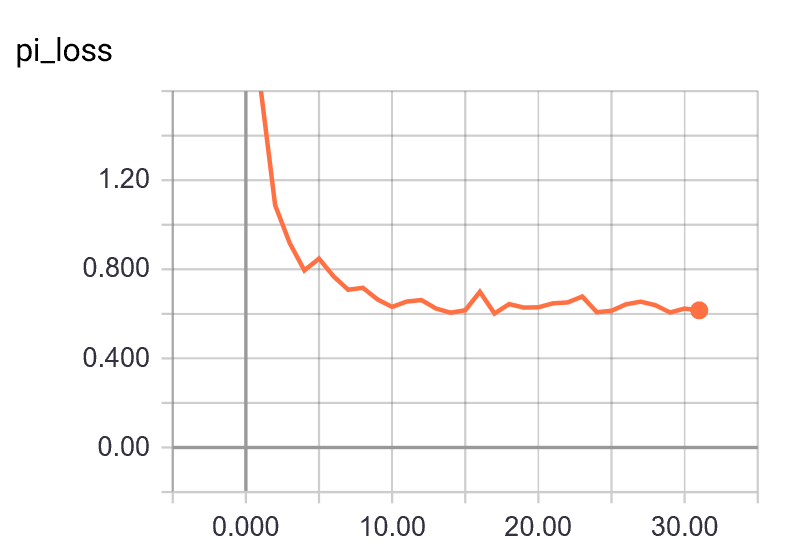
\includegraphics[width=0.3\linewidth]{pi_loss.png}
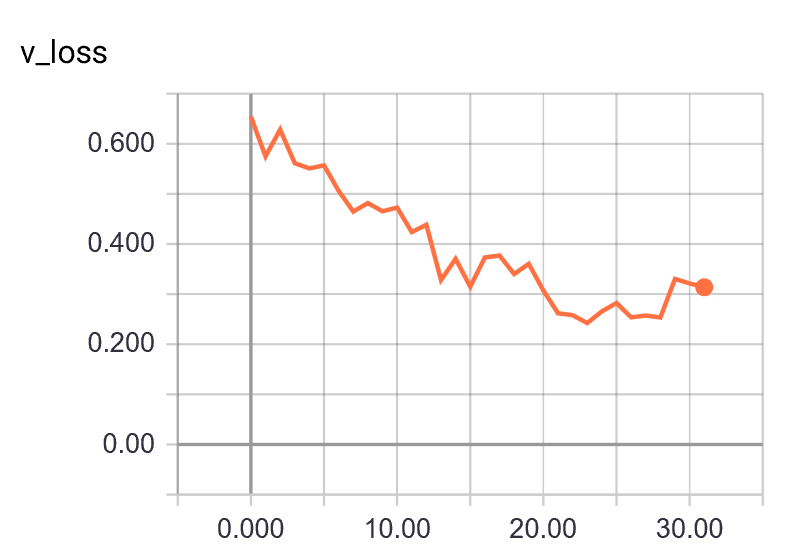
\includegraphics[width=0.3\linewidth]{value_loss.png}
\caption{Loss values after each epoch}
\end{figure}


\end{block}

%----------------------------------------------------------------------------------------

\end{column} % End of column 2.1

%----------------------------------------------------------------------------------------

\end{column} % End of column 2.1

\begin{column}{\onecolwid}\vspace{-.6in} % The second column within column 2 (column 2.2)

%----------------------------------------------------------------------------------------
%	METHODS
%----------------------------------------------------------------------------------------
\begin{column}{\onecolwid} % The second column within column 2 (column 2.2)

%----------------------------------------------------------------------------------------
%	RESULTS
%----------------------------------------------------------------------------------------

\begin{block}{Baseline Comparison}


\begin{figure}
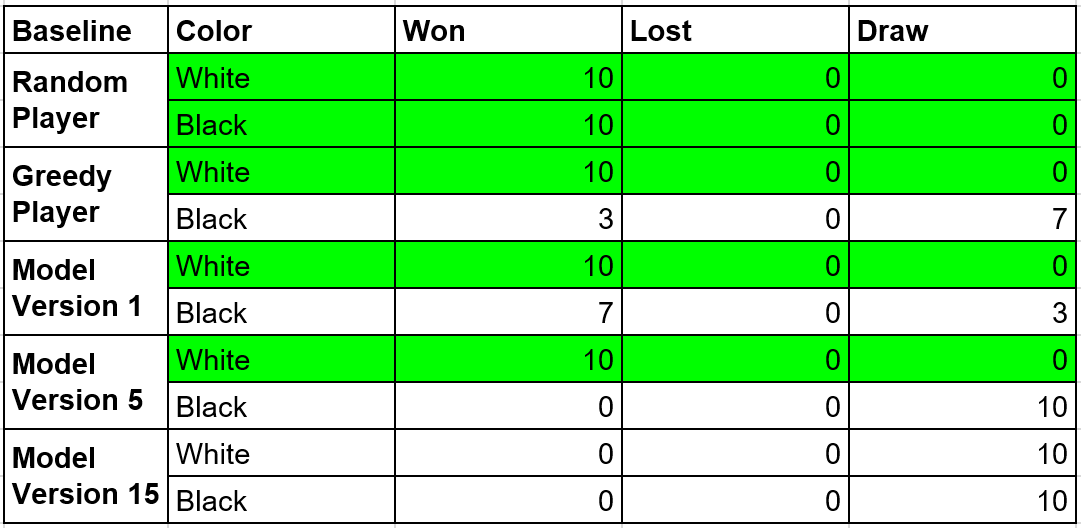
\includegraphics[width=0.8\linewidth]{baseline.png}
\caption{Results of pitting Best Model (V21) with other players}
\end{figure}

\begin{figure}
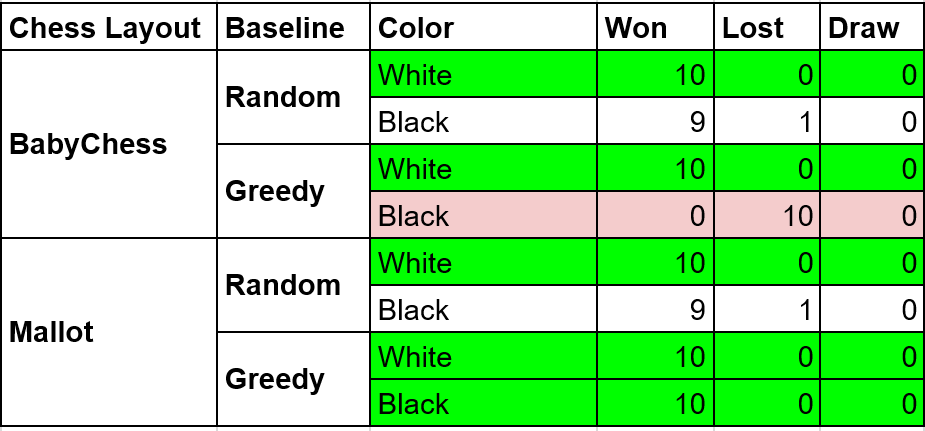
\includegraphics[width=0.7\linewidth]{diff_layouts.png}
\caption{Trained on Gardner and transferred to other layouts}
\end{figure}

\end{block}

%----------------------------------------------------------------------------------------

\end{column} % End of column 2.2

\begin{block}{Performance Improvements}

\begin{itemize}
\item 2.5 times improvement in training speed with distributed setup.
\end{itemize}
\begin{figure}
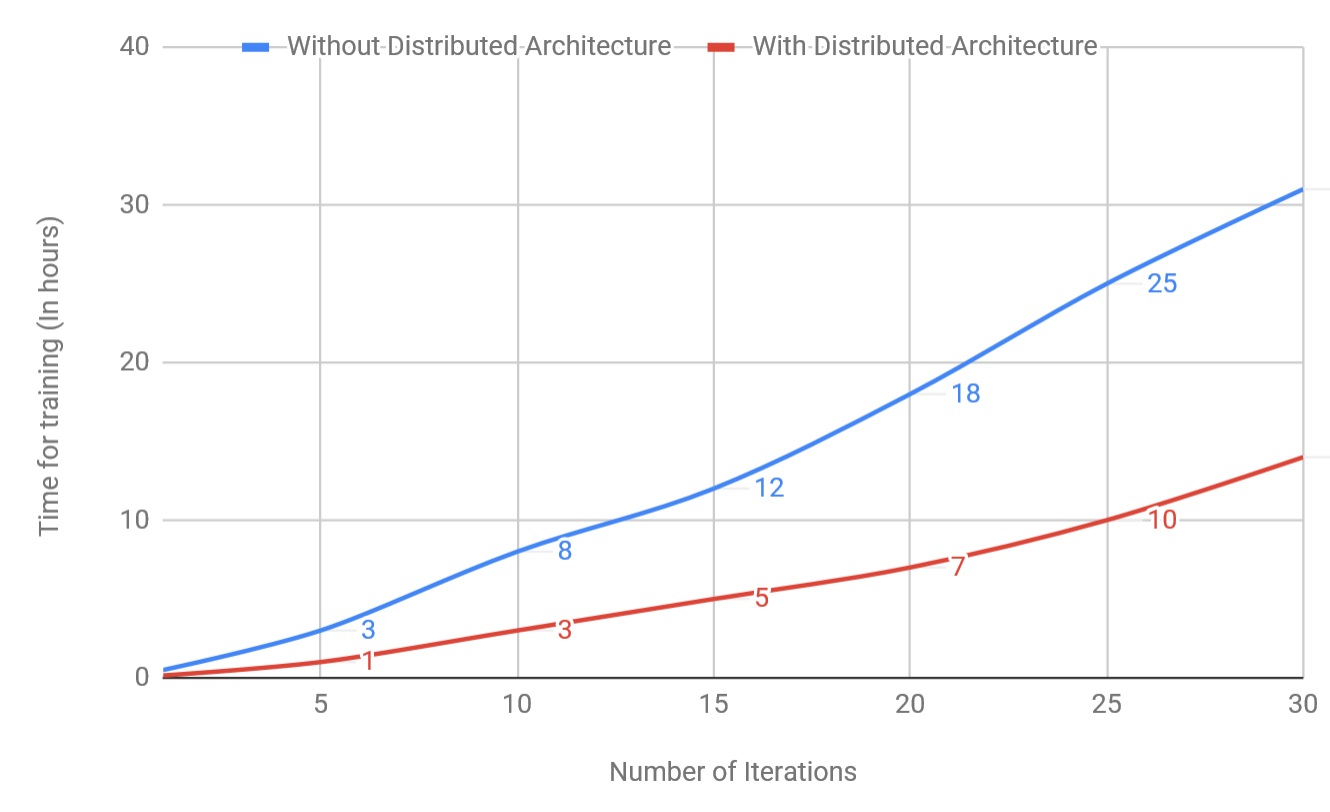
\includegraphics[width=0.7\linewidth]{performance_gain.png}
\caption{Single CPU vs Distributed Architecture}
\emph{After 21 iterations of training, when evaluated:}
\begin{itemize}
\item Defeats random player 100\%.
\item Defeats greedy player 100\% when Neural Net takes first turn (White)
\end{itemize}
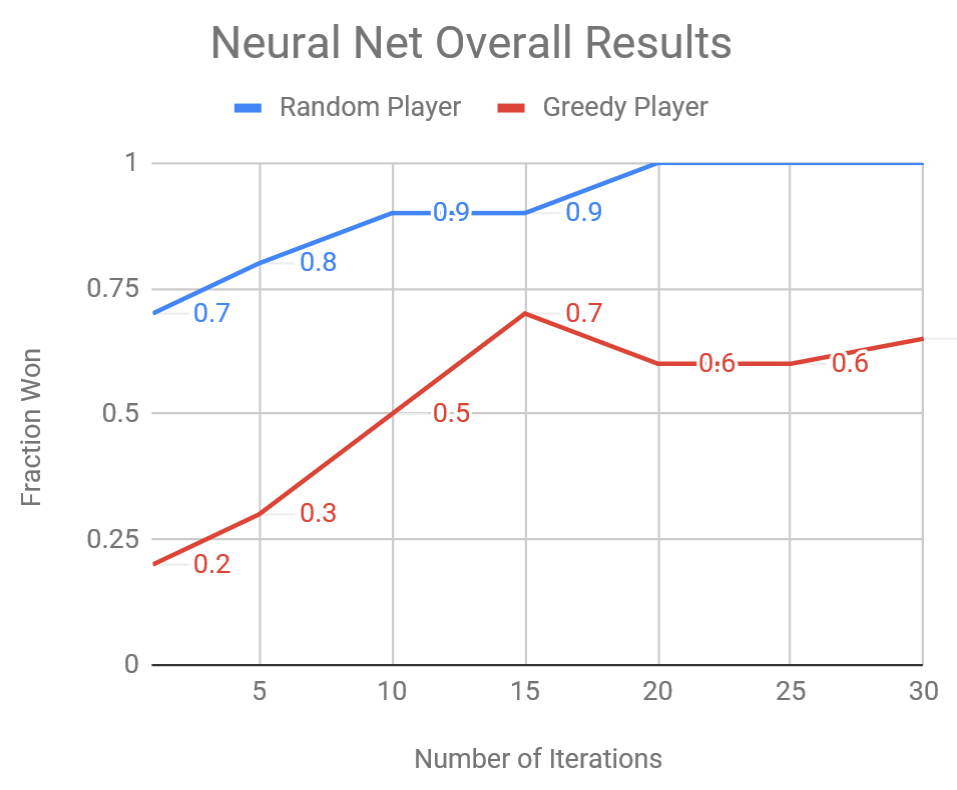
\includegraphics[width=0.3\linewidth]{neural_net_overall.png}
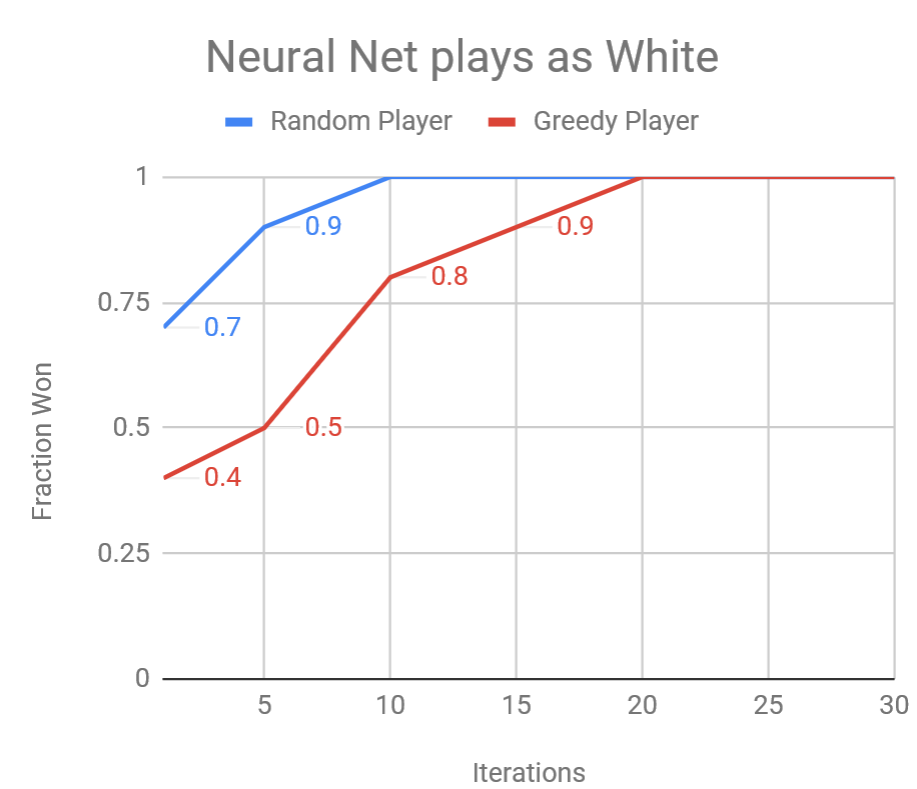
\includegraphics[width=0.3\linewidth]{neural_net_white.png}
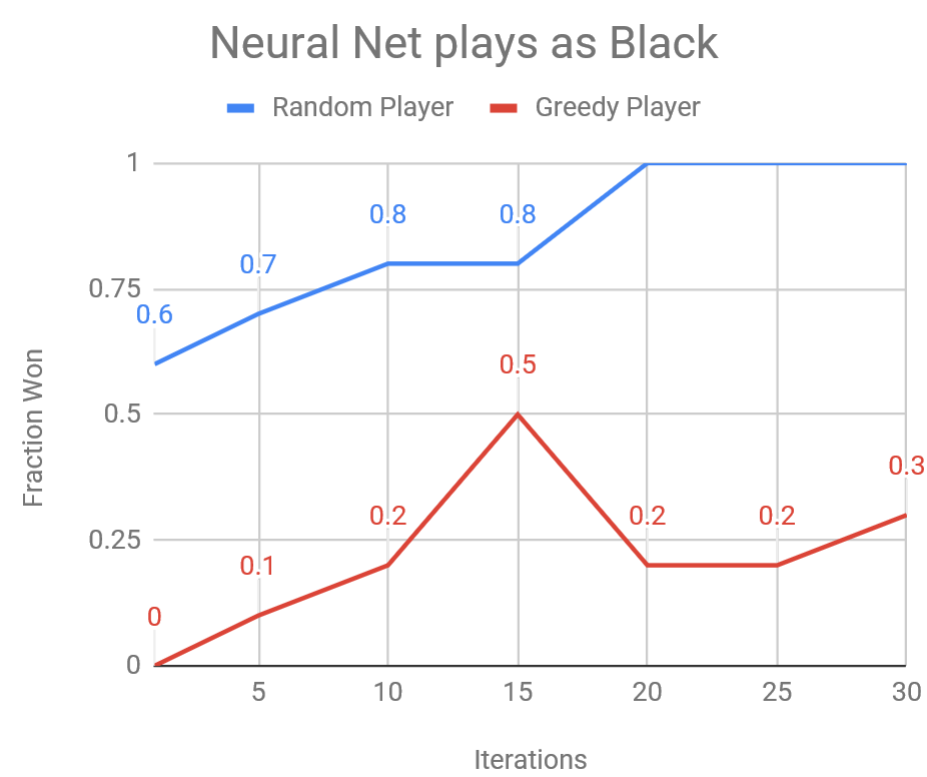
\includegraphics[width=0.3\linewidth]{neural_net_black.png}
\caption{Performance of Neural Net over other baselines}
\end{figure}

\end{block}

%----------------------------------------------------------------------------------------

\end{column} % End of column 2.2

\end{columns} % End of the split of column 2 - any content after this will now take up 2 columns width

%----------------------------------------------------------------------------------------
%	IMPORTANT RESULT
%----------------------------------------------------------------------------------------



%----------------------------------------------------------------------------------------

\begin{columns}[t,totalwidth=\twocolwid] % Split up the two columns wide column again




\end{columns} % End of the split of column 2

\end{column} % End of the second column

\begin{column}{\sepwid}\end{column} % Empty spacer column

\begin{column}{\onecolwid} % The third column


%----------------------------------------------------------------------------------------
%	CONCLUSION
%----------------------------------------------------------------------------------------

\begin{block}{Observations}

\begin{figure}
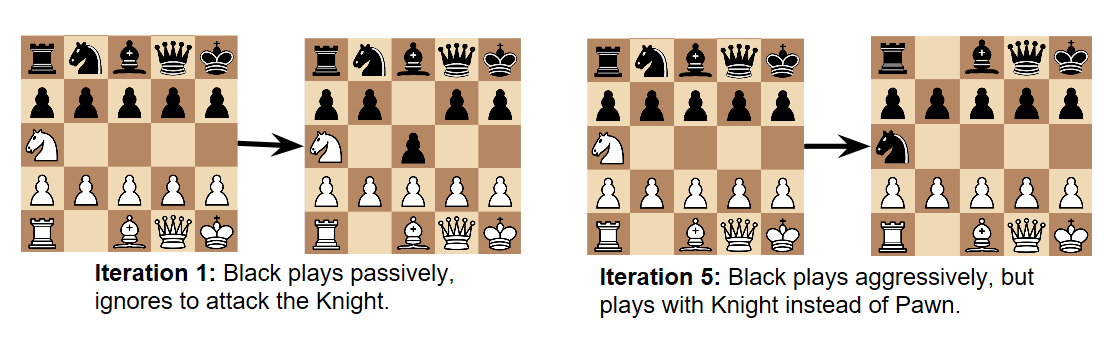
\includegraphics[width=1.0\linewidth]{attack_1.png}
\end{figure}


\begin{figure}
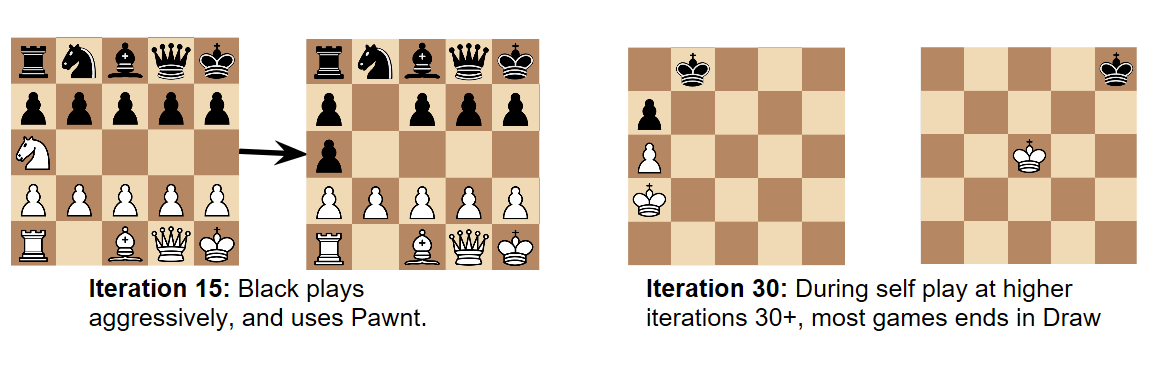
\includegraphics[width=1.0\linewidth]{attack_2.png}
\end{figure}


\end{block}


\begin{block}{Conclusion}

\begin{itemize}
\item Trained model beats the random, greedy baselines and performs decently on other layouts.
\item Monte Carlo Tree Search and CNN can approximate search space as large as $9 * 10^{18}$ as we seen in Minichess.
\item Parallelizing self play, training and pitter by leveraging cloud services improves the performance substantially
\end{itemize}

\end{block}

%----------------------------------------------------------------------------------------
%	ADDITIONAL INFORMATION
%----------------------------------------------------------------------------------------



%----------------------------------------------------------------------------------------
%	REFERENCES
%----------------------------------------------------------------------------------------

\begin{block}{References}


\begin{itemize}{}

\item Gardner's Minichess Variant is solved. Mehdi Mhalla et al. {\em arXiv e-print (arXiv:1307.7118) }
\item Learning to Play Othello Without Human Knowledge Surag Nair et al
\item Mastering Chess and Shogi by Self-Play with a General Reinforcement Learning Algorithm. Silver et al. 2017a
\end{itemize}

\end{block}

%----------------------------------------------------------------------------------------
%	ACKNOWLEDGEMENTS
%----------------------------------------------------------------------------------------



%----------------------------------------------------------------------------------------
%	CONTACT INFORMATION
%----------------------------------------------------------------------------------------


\begin{alertblock}{Contact Information}

\begin{itemize}
\item Web: \href{https://github.com/karthikselva/alpha-zero-general/tree/minichess}{https://github.com/karthikselva/alpha-zero-general/tree/minichess}
\item Demo Video: https://youtube.com/wahch?aw3rrfdf5
\item Mentor: patcho@stanford.edu
\end{itemize}

\end{alertblock}


%----------------------------------------------------------------------------------------

\end{column} % End of the third column

\end{columns} % End of all the columns in the poster

\end{frame} % End of the enclosing frame

\end{document}
